% \section{Introduction}
% Conventional classification methods in longitudinal analysis require sequences to be of uniform length~\cite{lu2018predicting} and without any missing records. This is rarely the case in data collected in the field and especially rare for data collected in the health care industry. In this section we explore one such dataset, and the difficulties it poses to existing classification methods, to discuss the merit of our proposed architecture.

% We consider a dataset of 375 samples, compiled from periodic blood-draws from COVID-19-positive patients during their stay at Tongji Hospital in China. These samples were collected during an outbreak of a pandemic, a time when hospitals function out of regular routine and blood draws are not necessarily performed for a controlled study. As a result, the number of blood draws is different for every patient and time intervals between samples are also often irregular. The data for this specific dataset was also conducted using CRFs (case report forms), or surveys filled out by individuals rather than being transcribed directly from a test result. The resultant inputs are uneven sequences of vectors with missing information that introduce several new difficulties, particularly when the missing information includes patient outcome, the target variable for any predictive model. 

% One might suggest imputation as a possible solution to the missing data problem. Modern imputation methods rely on a framework of generative adversarial networks (GANs)~\cite{yoon2018gain} to successfully impute sizeable portions of high-dimensional data. Although they are efficient, even state-of-the-art techniques assume records to be missing-at-random, an assumption that risks introducing unintended bias into a model. Alternatively, we could designate missing values with a recurring value, such as 0, and implement a model architecture that effectively ignores signal noise. Autoencoder is one such architecture that is frequently used to encode sequences, typically in a lower dimension, and could be used to learn temporal features from data. In longitudinal analysis, however, autoencoders assume an underlying time function, implied by uniform time intervals between records, that allows for unsupervised learning~\cite{langkvist2014review,srivastava2015unsupervised}. This assumption of a time function provides a powerful advantage to autoencoders, but also makes it impossible to learn from data that contains uneven sequences~\cite{yu2013embedding}, as might result from different patients receiving a different number of blood draws during their stay at a hospital. 

% We propose a semi-supervised Autoencoder (AE) enrichment method to encode a given sample's longitudinal information into a single fixed-length vector. For every sample, we create a LSTM cell consisting of a series of interconnected encoder-decoder pairs, one for each time stamp in the sample. The result is a fixed-length encoded vector, which can be fed into a predictor that learns such encodings. 

\IEEEraisesectionheading{\section{Introduction}\label{sec:introduction}}
\iffalse 
% and are usually filled with imputation techniques in a pre-processing phase [A. Farhangfar, L. Kurgan, and J. Dy. Impact of imputation of missing values on classification error for discrete data]. Furthermore, an imputation method may introduce a strong bias that influences the outcome of the analysis, especially for large fractions of missing values [R. J. A. Little and D. B. Rubin. Statistical Analysis with Missing Data.].
% Missing values in MTS are commonly found in domains such as healthcare and derive from measurement errors, incorrect data entry or lack of observations.

% Most patients had multiple blood samples taken throughout their stay in hospital. 
However, the model training and testing uses only the data from the final sample as inputs to the model to assess the crucial biomarkers of disease severity, distinguish patients that require immediate medical assistance and accurately match corresponding features to each label.[An interpretable mortality prediction model for COVID-19 patients]
% Missing data were ‘−1’ padded. 
% The model output corresponds to patient mortality. Patients that survived were assigned to class 0 and those that died to class 1.

As per the World Health Organisation, no vaccine and anti-viral treatments are yet available for this virus [Organization W.H., et al. Q&a on coronaviruses. 2020b.], and medical organisations are trying hard to find out the vaccine for this novel coronavirus.

Predicting mortality among patients with COVID-19 who present with a spectrum of complications is very difficult, hindering the prognostication and management of the disease.
The COVID-19 pandemic has affected more than 18 million individuals, and caused almost 700 000 deaths worldwide as of Aug 3, 2020.[Dong E, An interactive web-based dashboard to track COVID-19 in real time.]

At present, owing to the widespread nature of COVID-19, factories are being shut down, schools are being suspended, and people are isolating in their own homes, significantly disrupting daily life.

The emergence of COVID-19 has been a heavy burden.

The pandemic spread of coronavirus leads to increased burden on healthcare services worldwide. Experience shows that required medical treatment can reach limits at local clinics and fast and secure clinical assessment of the disease severity becomes vital. In L. Yan et al. a model is presented for predicting the mortality of COVID-19 patients from their biomarkers. 

The triage of coronavirus-19 patients into various strata based on some prognostic indicator might prove a utilitarian strategy in the management of epidemic. The goal of health-care facilities is optimization of the use of medical resources. The present study aimed to develop a predictor model of mortality risk from routine hematologic parameters. 
Coronavirus disease 2019 (COVID-19) is a disease caused by severe acute respiratory syndrome-coronavirus-2 (SARS-CoV-2). The emergence of the disease occurred in more than 200 countries of the world.[Worldometers. Available from: http://www.worldometers.info/coronavirus/. [Last accessed on 2020 May 22]]

A hospital-based, retrospective, case–control study was designed in the SMS Medical College and Hospital, Jaipur, to develop a prediction model for mortality risk using logistic regression analysis in COVID-19 patients. The patients were managed as per standard protocol of the institute. The study included case records of 23 nonsurvivors (33\%) and 47 survivors (67\%) with laboratory-confirmed SARS-CoV-2 infection. The demographic and laboratory details at the time of admission were collected to create database. The dependent variable was qualitative, either survivor or nonsurvivor. The regressors (or predictors) included age, gender, presence of symptoms, RBS, and complete blood count.[http://www.ijmbs.org/article.asp?issn=1947-489X;year=2020;volume=12;issue=2;spage=123;epage=129;aulast=Bhandari#ref1]

The novel coronavirus disease (COVID-19) spread rapidly throughout the world from Wuhan (Hubei, China) since December 2019 [Hu Y, et al. Clinical features of patients infected with 2019 novel coronavirus in Wuhan, China. The lancet.; Ou C-q, He J- x, et al. Clinical characteristics of coronavirus disease 2019 in China. New England journal of medicine.; Liu X, Zhang J, et al. Clinical characteristics of 138 hospitalized patients with 2019 novel coronavirus–infected pneumonia in Wuhan, China.]. The COVID-19 disease is caused by the severe acute respiratory syndrome coronavirus 2 (SARS-CoV-2), which is a member of the coronavirus family. On 11 March 2020, COVID-19 was declared as a pandemic by the World Health Organization (WHO). Due to the pandemic, hospital capacity is being exceeded in many places and face issues in terms of limited medical staff, personal protective equipment, life-support equipment and others [Cecconi M. Critical care utilization for the COVID-19 outbreak in Lombardy, Italy: early experience and forecast during an emergency response.; Sah P, Pandey A, et al. Projecting hospital utilization during the COVID-19 outbreaks in the United States.].
This can be avoided by prioritizing hospital treatment for patients at high risk of deterioration and death, and treating low-risk patients in ambulatory environments, or by home-based self-quarantine. An effective tool is required to predict the disease trajectory to allocate resources efficiently and also improve the patient’s condition. In other words, early identification of patients at high risk for progression to severe COVID-19 will help in efficient utilization of healthcare resources via patient prioritization to reduce the mortality rate.

The world would remember the year 2020 as a catastrophic year for humanity on this planet earth.

Specifically, we consider a semi-supervised learning methodology based on AutoEncoders to first extract the infected legions in chest X-ray manifestation of COVID-19 and other Pneumonia-like diseases (as well as healthy cases). 
Furthermore, the semi-supervised nature of the proposed framework enables us to efficiently exploit the limited available dataset on COVID-19 while exploiting the vast amount of available X-ray dataset for healthy and non-COVID classes. 
The proposed methodology can be seen as an amalgamation of supervised and unsupervised learning methodologies

% The AE is a neural network traditionally conceived as a non-linear dimensionality reduction algorithm [hinton2006reducing], which has been further exploited to learn representations in deep architectures [bengio2009learning].

% RNN was unable to model long term dependencies resulting LSTM came into picture and was introduced by Hochreiter et al. in 1997 [schmidhuber1997long].
Deep learning speculates that a deep sequential or hierarchical model is more efficient in classification or regression tasks than shallow models [Bengio Y. Learning deep architectures for ai.]. Recurrent neural networks contain hidden states distributed across time, and this allows them to store a lot of information about the past. They are most commonly used in forecasting applications due to their ability to process variable length sequential data [Graves A.. Generating sequences with recurrent neural networks.].

Furthermore, we conduct a comparison with other reported regression baselines and reference models that solve the same problems using the same datasets, indicating a clear superiority of the proposed approach using three different performance metrics. The main contributions of this paper are as follows:
Present a new LSTM-based autoencoder learning approach to solve
In fact, the latter approach has many advantages, such as conducting learning based on unlabeled data, and having the availability and abundance of unlabelled data, in contrast to labelled data.

% Recurrent neural networks have major disadvantage that they cannot overcome vanishing gradient or exploding gradient problem and also they can store only short-term memory because they involve hidden layer activation functions of the previous time step only [schmidhuber1997long].
\fi
%%%%%%%%%%%%%%%%%%%%%%%%%%%%%%%%%%%%%%%%%%%%%%%%%%%%%%%%%%%%%%%%%%%%%%%%%%%%%%%%%%%
%% begin - IB
% Sudden increases in COVID-19 cases, such as during seasonal waves, quickly
% deplete the limited resources of healthcare systems~\cite{kontis2020magnitude}, forcing clinicians to set
% criteria for distribution of scarce treatments, such as N95
% respirators~\cite{centers2020strategies}. In an earlier study, Yan et al. advocated for
% a machine learning mortality-prediction model to inform logistical
% planning~\cite{yan2020interpretable}.  The model proposed in the study takes in data from
% patients' blood samples to identify the most predictive biomarkers using
% a XGBoost classifier algorithm. This data was obtained from a publicly available
% dataset whose samples were collected using case report forms (CRFs) and
% contained longitudinal records on 358 COVID-19-positive patients admitted to
% Tongji Hospital in China. Most patient samples also contained a `patient
% outcome' feature, which the model could use as a target variable. Acknowledging
% the limitations of XGBoost classifier models in taking in misaligned temporal data,
% only the final record from each patient was used to train and test the model.
% While this technique accomplished the task of deter- mining the most predictive
% biomarkers, it failed to capture change in time, a feature central to the
% progression of COVID-19. In this study, we attempt a similar classification
% task on this same dataset, but with the goal of producing a general predictive
% model that incorporates temporal features into its predictions.

% Conventional classification methods in MTS analysis require vector
% sequences of fixed length, which is rarely the case when data is collected
% outside of a carefully controlled environment. Our samples were collected
% during an outbreak of a pandemic, a time when hospitals function out of routine
% blood draws are not performed with for a controlled study. As a result, the
% number of blood draws different for every patient and  time intervals between
% samples are also often irregular. The data for this specific dataset was also
% conducted using CRFs, or surveys filled out by individuals rather than being
% transcribed directly from a test result. The resultant inputs are uneven
% sequences of vectors with missing information that introduce several new
% difficulties, particularly when missing the missing information includes
% patient outcome, the target variable for any predictive model.

% One might suggest imputation as a possible solution, at least to tackle missing
% the missing data problem. Modern imputation methods rely on a framework of
% generative adversarial networks (GANs)~\cite{yoon2018gain} to successfully impute
% sizeable portions of high-dimensional data. Although they are efficient, even
% state-of-the-art techniques assume records to be missing-at-random, an
% assumption that risks introducing unintended bias into a model. If we suppose
% that the data is perfectly imputed and that we are able to coerce
% a classification model to recognize time as a feature, there is still
% variability within individual samples. Patient blood is sampled only when
% the clinician deems it necessary, so the number of records in a sequence, as
% well as the time interval between samples, is most likely different for every patient.
% Many MTS models require the number of the records to be uniform across
% sequences while techniques that are reliant on time underlying time functions,
% such as autoencoders, fail completely when the intervals between records are
% non-uniform~\cite{yu2013embedding}. All of these difficulties are typically tackled by
% removing samples, a practice that leads to a smaller dataset and a less
% accurate model.
%% end - IB
\IEEEPARstart{S}{udden} increases in COVID-19 cases, such as during seasonal waves, quickly deplete the limited resources of health care systems, forcing clinicians to set criteria for distribution of scarce treatments~\cite{centersstrategies}. In an earlier study, Yan et al. advocated for a machine learning mortality-prediction model to inform logistical planning~\cite{yan2020interpretable}. The model~\cite{yan2020interpretable} proposed in the study identifies the most predictive biomarkers for the patient's mortality using a XGBoost classifier~\cite{chen2016xgboost} trained on a publicly available MTS dataset collected from COVID-19-positive patients admitted to Tongji Hospital in China. Acknowledging the limitations of the random XGBoost classifier in synthesizing longitudinal data, only the final record was used to train and test the model. While the model accomplishes the task of determining the most predictive biomarkers, it hardly captures the temporal trends, which are crucial to capturing the progression of this disease. In addition, the model is not able to predict the mortality when these principle biomarkers are not measured.
% [It is an acute public health crisis leading to overloaded critical care capacity. Timely prediction of the clinical outcome (death/survival) of hospital-admitted COVID-19 patients can provide early warnings to clinicians, allowing improved allocation of medical resources.COVID-19 pandemic has created an extreme pressure on the global healthcare services. Fast, reliable and early clinical assessment of the severity of the disease can help in allocating and prioritizing resources to reduce mortality.]

To learn the relationships across variables and time steps, MTS analysis models have be proposed. The samples from COVID-19 patients were collected during an outbreak of a pandemic, a time when hospitals function out of routine and blood draws are not performed for a controlled study. As a result, the number of blood draws is different for every patient and time intervals between samples are often irregular. The resultant inputs are uneven sequences of vectors with missing data that is difficult to be integrated with the static data represented by a fixed length vector. However, conventional MTS analysis usually require sequences to be complete and of consistent length~\cite{lu2018predicting,wang2017longitudinal,wang2016prediction,wang2012high}, which is rarely the case when data is collected outside of a carefully controlled environment. In addition they often do not integrate static and dynamic data from different modalities to improve prediction.

% The data for this specific dataset was also collected from CRFs (case report forms), or surveys filled out by individuals rather than being transcribed directly from a test result.
% The resultant inputs are uneven sequences of vectors with missing data that introduce several new difficulties, particularly when the missing data includes patient outcome, the target variable of predictive model. One might suggest imputation as a possible solution, at least to tackle the missing data problem. Modern imputation methods rely on a framework of generative adversarial networks (GANs)~\cite{yoon2018gain} to successfully impute sizeable portions of high-dimensional data. Although they are efficient, the imputation may introduce undesirable bias in prediction.
% [In case of missing data, the whole observation has been removed from the analysis.[http://www.ijmbs.org/article.asp?issn=1947-489X;year=2020;volume=12;issue=2;spage=123;epage=129;aulast=Bhandari#ref1]]
% Although they are efficient, even state-of-the-art techniques assume records to be missing-at-random, an assumption that risks introducing unintended bias into a model. If we suppose that the data is perfectly imputed and that we are able to coerce a classification model to recognize time as a feature, there is still variability within individual samples. Patient's blood is sampled only when the clinician deems it necessary, so the number of records in a sequence, as well as the time interval between samples, is most likely different for every patient. Many MTS models require the number of the records to be uniform across sequences while techniques that are reliant on time underlying time functions, such as autoencoders, fail completely when the intervals between records are non-uniform~\cite{yu2013embedding}. All of these difficulties are typically tackled by removing samples, a practice that leads to a smaller dataset and a less accurate model. 
% XGBoost -> conventional longitudinal/missing data -> deep learning LSTM / unlabeled data -> LSTM autoencoder / fixed-length vector which is not longitudinal anymore -> our model.

To overcome the problems from missing data and an inconsistent number of records, recurrent neural networks (RNNs)~\cite{medsker2001recurrent}, especially Long Short Term Memory (LSTM)~\cite{schmidhuber1997long}, have been successfully applied in MTS analysis. Due to their flexibility in handling missing data and ability to learn long-term dependencies, they achieve state of the art results in supervised learning tasks involving MTS with large numbers of records. However, due to the fact that a significant portion of COVID-19 patient's records are collected in the field and are unlabeled, supervised learning models may not be efficient and practical tools in the prediction of clinical outcomes of COVID-19 patients.

Recent unsupervised learning models~\cite{srivastava2015unsupervised,langkvist2014review,saumya2020spam,hinton2006reducing} have leveraged RNNs to learn the representation of MTS in a lower dimensional space. A proper representation of MTS data is crucial because MTS usually contains noises and redundant information from the large number of features and records~\cite{tuncel2018autoregressive,langkvist2014review}. However, existing RNN models encode MTS into the other longitudinal enriched representations which are difficult to be integrated with the static data, such as demographic or genetic information. Another disadvantage of existing unsupervised representation learning models is they often do not utilize labeled samples, when the target labels of samples can improve the representation learning for better predictions.

Therefore, we propose an alternate solution in the form of a novel LSTM autoencoder architecture to transform the incomplete MTS into a vectorial representation which can be readily integrated with the static data. Unlike the previous LSTM autoencoder models in~\cite{srivastava2015unsupervised,langkvist2014review,saumya2020spam}, the proposed model encodes the MTS into a fixed length vector which is no longer longitudinal. Considering that the data collected in the field usually consists of labeled and unlabeled samples, the proposed semi-supervised learning model utilizes both, improving predictions compared to the strictly supervised~\cite{yan2020interpretable} or unsupervised~\cite{langkvist2014review,srivastava2015unsupervised} learning models. In our experiments with two MTS datasets, we show that the learned representation helps improve predictions on mortality of patients, especially when only a small proportion of samples are labeled. The proposed prediction model will be useful for improving the speed of triage and resource distribution.
% \begin{figure}
%     \centering
%     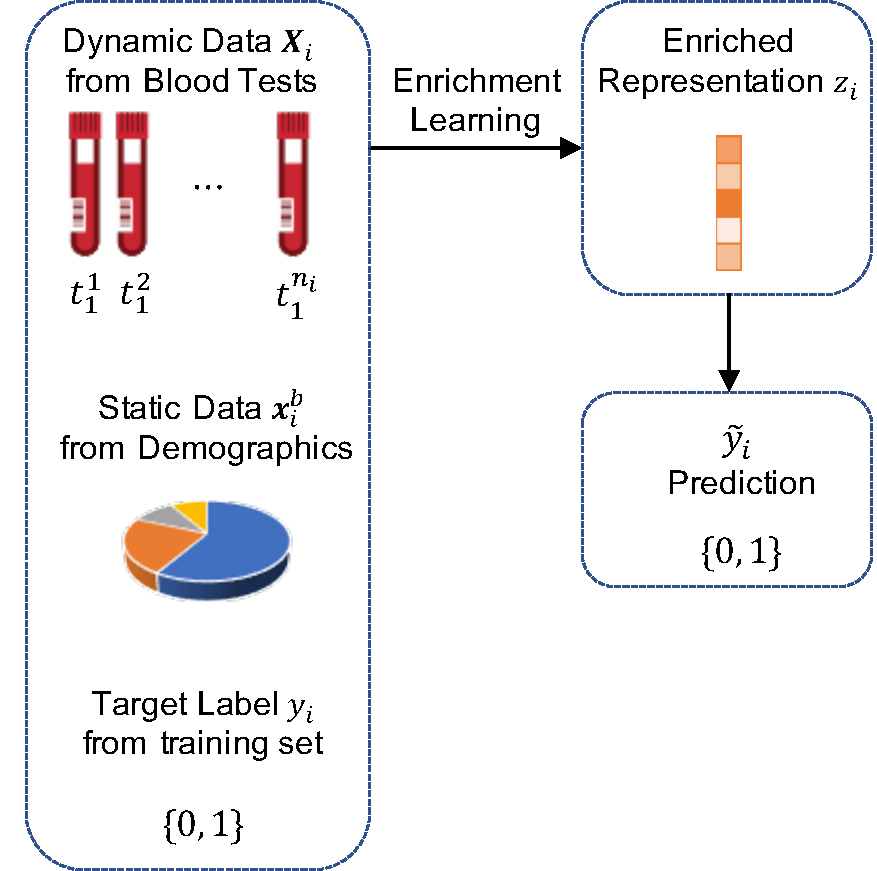
\includegraphics[width=1.0\linewidth]{figures/enrichment-learning.pdf}
%     \caption{The prediction via enrichment. MTS with uneven time intervals and missing data is represented by the sparse matrix $\mathbf{X}_i$ of varying size. We first compress the matrix of MTS into the enriched representation in a fixed length vector format, and then predict target labels from the enriched vectorial representation.} \label{fig: enrichment-learning}
% \end{figure}

% [A proper representation of the data is crucial in machine learning applications [Y. Li, S. Wang, Q. Tian, and X. Ding. Feature representation for statistical-learning-based object detection:].]
% [Traditionally, autoencoders are used for generating a compressed representation of the input by projecting it into a dense low dimensional space.]

% [The decoder LSTM is being asked to reconstruct back the input sequence from this representation. In order to do so, the representation must retain information about the appearance of the objects and the background as well as the motion contained in the video.]
% [Under these circumstances, we retrospectively analysed the blood samples of 385 patients from the region of Wuhan, China, to identify robust and meaningful markers of mortality risk. 38=75(training set) + 110(test set).]
% [The proposed prediction model may be helpful for the quick triage of patients without having to wait for the results of additional tests such as laboratory or radiologic studies, during a pandemic when limited medical resources must be wisely allocated without hesitation.]
% Our model uses an encoder LSTM to map an input sequence into a fixed length representation.
% For unlabeled data, still learns how to summarize the records by minimizing reconstruction error. And this enhanced summarization capability helps prediction.

% Text Here. However, existing RNN based Autoencoders has a RNN decoder [Filippo Maria Bianchi, Learning representations of multivariate MTS with missing data] [Nitish Srivastava, Unsupervised Learning of Video Representations using LSTMs], and they are supervised learning methods. By providing mask vector, encoder can utilize the missingness pattern [the missingness patterns might be useful to characterize the data]. [Results confirm that our method significantly improves the quality of the representations as the percentage of un-labeled samples increases.]. Because COVID-19 is novel virus, there is not enough mortality labeled data. 
% Pre-trained model can be used to new data in real time, without cold start problem.

% \subsection{Contribution}
% Text Here.

% \subsection{Paper Organization}
% Text Here.

% The previous researches \cite{hinton2006reducing,yu2013embedding} have been constructed encoder with neural network as a non-linear dimensionality reduction tool. When it comes to longitudinal records of MTS dataset, Recurrent Neural Network (RNN) has successfully learned representations retaining important temporal trends to reconstruct the original longitudinal records~\cite{hinton2006reducing}. However, RNN has been criticized as it suffers from vanishing or exploding gradient problem and it cannot learn the long term dependencies~\cite{schmidhuber1997long}. More recently, LSTM has been emerged 
% and to deal with these problems, LSTM has been emerged~\cite{schmidhuber1997long}. Because it is crucial to learn the long term temporal trends along the patient's records, we leverage LSTM to encode the patient's records. 

%% The current reconstruction can be biased by the previous reconstruction which does not contain any useful information.

%% The previous study used LSTM for encoder and decoder both, and copied enriched vectorial representation along $n_i$ times points to feed the LSTM decoder because LSTM requires the input to be sequence of $n_i$ records. As a result, the reconstruction at $j$-th time step depends on the reconstruction at $j-1$-th time step. However, because the actual input of decoder is a single vector, no information is additionally provided for each time step, thus the reconstruction of current time step should not be biased by the reconstruction of previous time step. 